\documentclass[../main.tex]{subfiles}
\begin{document}
\chapter{Natural Numbers and Counting}
\section{Natural Numbers}
\begin{definition}[Natural Numbers]
  \label{naturalDef}
  The natural numbers $\N$ is a set containing the special element ``1'', together with a map $S: \N \to \N$ called the ``successor function'' that maps $n \in \N$ to its successor such that the following properties hold:
  \begin{enumerate}
    \item $\forall n \in \N, S(n) \neq 1$ (1 is not the successor of anything)
    \item $\forall m, n \in \N, S(m) = S(n) \implies m = n$ ($S$ is injective)
    \item Let $A$ be a subset of $\N$ such that $1 \in A$ and $n \in A \implies S(n) \in A$. Then $A = \N$.
  \end{enumerate}
\end{definition}
These are called the ``Peano Axioms''.
We also define the usual Arabic numeral system:
\[
  2 = S(1), 3 = S(2), 4 = S(3) \ldots
\]

We can also define addition recursively by:
\begin{itemize}
  \item $n + 1 = S(n)$
  \item $n + S(m) = S(n + m)$
\end{itemize}
Similarly for multiplication:
\begin{itemize}
  \item $n \times 1 = n$
  \item $n \times S(m) = n \times m + n$
\end{itemize}
For comparison we define $a < b$ if $\exists c$ such that $a + c = b$.
One key feature of $<$ is that for $m \neq n$ exactly one of $m < n$ or $n < m$.
\begin{example}
  For example, if we were to suppose $1 < 2$ and $2 < 1$ then  $\exists k, e$ s.t. $1 = 2 + k$ and $2 = 1 + e$ so $1 = 1 + e + k = S(e + k)$ but this contradicts the fact that 1 is not the successor of any number.
\end{example}

We can show that these operations satisfy the usual rules of arithmetic:
\begin{proposition}[Properties of Natural Numbers]
For all natural numbers:
  \begin{itemize}
    \item Addition and multiplication are commutative and associative
    \item Multiplication is distributive over addition
    \item $a < b \implies a + c < b + c$
    \item $a < b \implies a \times c < b \times c$
    \item if $a < b$ and $b < c$ then $a < c$
    \item $a < a$ is never true
  \end{itemize}
\end{proposition}
\begin{example}
  For example, to show that $1 + 2 = 2 + 1$ using the Peano axioms:
  \[
    1 + 2 = 1 + S(1) = S(1 + 1) = S(S(1)) = S(1) + 1 = 2 + 1
  \]
\end{example}
\begin{example}
  To show $n + m = m + n$ we would have to carry out induction both on $m$ and $n$.
\end{example}

\subsection{Induction}
\begin{definition}[Weak Principle of Induction - WPI]
  If $P(1)$ holds, and $\forall n \in N, P(n) \implies P(n + 1)$, then $P(n)$ holds $\forall n \in \N$.
\end{definition}
\begin{remark}[Note]
  WPI is equivalent to the third Peano Axiom (see \cref{naturalDef})
\end{remark}
There is also a different form of induction based on the ordering above:
\begin{definition}[Strong Principle of Induction - SPI]
  If $P(1)$ holds, and $\forall n \in N$, if $P(k)$ true $\forall k \leq n \implies P(n + 1)$, then $P(n)$ holds $\forall n \in \N$.
\end{definition}
Clearly $\text{SPI} \implies \text{WPI}$ as WPI is a less restrictive statement.
To see $\text{WPI} \implies \text{SPI}$ apply WPI to the statement $Q(n) =$ ``$P(k) \text{ holds } \forall k \leq n$''.

The above ordering of $\N$ satisfies a special property called the ``Well Ordering Principle'' (WOP).
\begin{definition}[Well Ordering Principle - WOP]
  Every non-empty subset of the natural numbers has a minimal element.
  That is, if $P(n)$ holds $\forall n \in  A \subset \N$ with $A \neq \emptyset$ then there exists a least $m \in A$ such that $P(m)$ holds.
\end{definition}
\begin{theorem}
  $\text{SPI} \implies \text{WPI}$.
\end{theorem}
\begin{proof}
  Suppose $P(n)$ holds for some non-empty subset of the naturals and, for contradiction, that there is in fact no least $n \in \N$ such that $P(n)$ holds.

  Consider $Q(n) = \lnot P(n)$.
  Certainly $P(1)$ is false else $1$ would be the minimal element, so $Q(1)$ is true.

  Given some $n \in \N$, suppose $Q(k)$ is true $\forall k < n$.
  Then $P(k)$ is false $\forall k < n$ so $P(n)$ must be false as otherwise $n$ would be the minimal element.
  But this means that $Q(n)$ is true.

  Both conditions of the SPI are satisfied so $Q(n)$ holds $\forall n \in \N$.
  So $P(n)$ is false $\forall n \in \N$ which contradicts the fact that $P(n)$ holds for a non-empty subset of the naturals.
\end{proof}
\begin{remark}
  $\text{WOP} \centernot\implies \text{SPI}$.
  However in most proofs using SPI, you can in fact use WOP.
\end{remark}
\begin{example}
  Any natural number $>1$ can be written as a product of primes (Fundamental Theorem of Arithmetic)
\end{example}
\begin{proof}[Proof Using WOP]
  Let $C$ be the set of counter examples, that is:
  \[
    C = \{n \in \N: n > 1, n \text{ cannot be written as a product of primes}\}
  \]
  For contradiction, we assume that $C \neq \emptyset$.
  By WOP, $C$ has a least element $m$.
  Clearly $m$ must be composite, so $m = ab$ with $1 < a, b < m$.
  So at least one of $a$ or $b$ does not have a prime factorisation, WLOG, suppose $a$ does not have a prime factorisation.
  This means $a \in C$, but $a < m$ so this contradicts the fact that $m$ is the minimal element of $C$.
\end{proof}
\section{Counting Sets}
\subsection{Power Sets}
\begin{remark}[Reminder]
  Recall that a set $A$ has \textit{size} $n$ if we can write $A = \{a_1, a_2, \ldots, a_n\}$ with the elements $a_i$ distinct.
  We write $|A| = n$.
  We say $A$ is finite if the exists $n \in \N_0$ such that $|A| = n$, and $A$ is infinite otherwise.
  See \cref{finiteSets}.
\end{remark}
\begin{proposition}
  A set of size $n$ has exactly $2^{n}$ subsets.
\end{proposition}
\begin{proof}
  \induction
  {$n = 0$}{
    Clearly true for $n = 0$ as $\emptyset$ has 1 subset.
  }
  {$n = k - 1$}{
    So a set of size $k - 1$ has $2^{k - 1}$ subsets.
  }
  {$n = k$}{
    Given $n > 0$ and $T \subseteq \{1, 2, \ldots, n - 1\}$, how many subsets $S \subseteq \{1, 2, \ldots, n\}$ are there such that $S \cap \{1, 2, \ldots, n - 1\} = T$.
    There are exactly 2, namely $T$ and $T \cup \{n\}$.
    Hence the number of subsets of $\{1, 2, \ldots, n\}$ is twice the number of subsets of $\{1, 2, \ldots, n - 1\}$. Which is $2 \times 2^{n - 1} = 2^{n}$ by the inductive hypothesis.
  }
\end{proof}
\begin{corollary}
  $|\powerset{A}| = 2^{|A|}$.
\end{corollary}
\begin{proof}
  $\powerset{A}$ is the set of all subsets of $A$ so must have size $2^{|A|}$.
\end{proof}

\subsection{Binomial Coefficients}
\begin{definition}[Binomial Coefficient]
  Given $n \in \N_0$ and $0 \leq k \leq n$ we write $\binom{n}{k}$ for the number of subsets of an $n$-element set that are of size k.
  That is:
  \[
    \binom{n}{k} = \abs{\{S \subseteq \{1, 2, \ldots, n\} : |S| = k\}}
  \]
  This is often called the \textit{choose function} and said ``$n$ choose $k$''.
\end{definition}
\begin{example}
  The subsets of size 2 of $\{1, 2, 3, 4\}$ are:
  \[
    \{1, 2\}, \{1, 3\}, \{1, 4\}, \{2, 3\}, \{2, 4\}. \{3, 4\}
  \]
  So $\binom{4}{2} = 6$
\end{example}
By definition $\binom{n}{0} = 1$, $\binom{n}{n} = 1$ , $\binom{n}{1}$ for $n > 0$.

As the total number of subsets is $2^{n}$ we have that:
\[
  \binom{n}{0} + \binom{n}{1} + \binom{n}{2} + \cdots + \binom{n}{n-1} + \binom{n}{n} = 2^{n}
\]

We also have:
\[
  \binom{n}{k} = \binom{n}{n - k} \quad \forall n, k \in \N_0,\ 0 \leq k \leq n
\]
This is because specifying which $k$ elements to pick is the same as specifying which $n - k$ elements \textit{not} to pick.

Moreover:
\[
  \binom{n}{k} = \binom{n - 1}{k - 1} + \binom{n - 1}{k} \quad \forall n, k  \in \N,\ 0 < k < n
\]
This is the same as saying we either include some special element and have $k - 1$ elements left to pick from $n - 1$ or we exclude the special element and have $k$ elements left to pick from $n - 1$.

From this identity we can obtain \textit{Pascal's triangle}:
\begin{center}
\begin{tikzpicture}[scale=1.0, every node/.style={font=\footnotesize}]
\def\n{6}
\def\ysep{0.4}

\pgfmathsetmacro{\xoffset}{-\n/2 - 0.3}

\foreach \row in {0,...,\numexpr\n-1} {
    \node[anchor=east] at (\xoffset, -\row*\ysep) {$n=\row$};

    \foreach \col in {0,...,\row} {
        \pgfmathparse{int(factorial(\row)/(factorial(\col)*factorial(\row-\col)))}
        \let\binom=\pgfmathresult
        \node at ($(-\row/2+\col, -\row*\ysep)$) {\binom};
    }
}

\draw[<-] (-3/2 + 2 + 0.2, -\ysep * 3) -- (3.5, -0.5) node[right] {$\binom{3}{2}$};
\end{tikzpicture}
\end{center}
Each row starts and ends with 1, and the other remaining remaining entries are the sum of the two terms directly above.
Indexing from 0, the $k$-th element of the $n$-th row is $\binom{n}{k}$.
\begin{proposition}
  The following formula can be used to directly compute binomial coefficients:
  \[
    \binom{n}{k} = \frac{n(n-1)(n-2)\cdots(n-k+1)}{k(k-1)(k-2)\cdots2\cdot1} = \frac{n!}{k!(n - k)!}
  \]
\end{proposition}
\begin{proof}
  Given a set of size $n$, there are $n$ ways to pick the first element, $n - 1$ ways to pick the second element and so on.
  So there are $n(n-1)(n-2)\cdots(n-k + 1)$ ways to pick $k$ elements in order.

  But each subset of size $k$ is picked in $k(k-1)(k-2)\cdots2\cdot1$ ways by this method.
  Hence the number of subsets of size $k$ in a set of size $n$ is exactly:
  \[
    \frac{n(n-1)(n-2)\cdots(n-k+1)}{k(k-1)(k-2)\cdots2\cdot1} = \frac{n!}{k!(n - k)!}
  \]
\end{proof}
\begin{remark}[Note]
  The formula tells us, for example, that $\binom{n}{2} = \frac{1}{2}n(n-1) \sim \frac{1}{2}n^2$.
  Similarly for $\binom{n}{3} = \frac{1}{6}n(n-1)(n-2) \sim \frac{1}{6}n^3$.
\end{remark}
\begin{remark}[Notation]
  $\sim$ denotes the asymptotic behaviour of an expression for large $n$.
\end{remark}
\begin{theorem}[Binomial Theorem]
  For all $a, b \in \R$, $n \in \N$:
  \begin{align*}
    (a + b)^{n} &= \binom{n}{0}a^{n} + \binom{n}{1}a^{n - 1}b + \binom{n}{2}a^{n-2}b^{2} + \cdots + \binom{n}{n-1}ab^{n-1} + \binom{n}{n}b^{n} \\
                &=\sum_{k=0}^{n} \binom{n}{k}a^{n - k} b^{k}
  \end{align*}
\end{theorem}
\begin{proof}
  When we expand $(a + b)^{n}$:
  \[
    (a+b)^{n} = \underbrace{(a + b)(a + b)(a + b) \cdots (a + b)}_{n \text{ terms}}
  \]
  we obtain terms of the form $a^{n - k}b^{k}$, $0 \leq k \leq n$.
  The number of terms of this form is exactly $\binom{n}{k}$ because we have to select $k$ brackets from $n$ brackets from which to pick $b$.
  Hence $(a + b)^{n} = \sum_{k=0}^{n} \binom{n}{k}a^{n - k}b^{k}$.
\end{proof}
\begin{example}[Making Approximations]
  Consider:
  \[
    (1 + x)^{n} = 1 + nx + \frac{n(n-1)}{2}x^2 + \binom{n}{3}x^3 + \cdots + \binom{n}{n-1}x^{n-1} + x^{n}
  \]
  so for small $x$, a good approximation to $(1 + x)^{n}$ is just some truncated part of this expression.

  For example, $1 + nx$, so $(1.00001)^{8} \approx 1.00008$.
  If we wanted a better approximation we could instead use $1 + nx + \frac{n(n-1)}{2}x^2$, so $(1.00001)^{8} \approx 1.00008 + 28 \cdot (0.00001)^{2}$.
\end{example}
\subsection{Inclusion Exclusion Principle}
What can we say about the relationships between sizes of unions and intersections of finite sets?
For example, to find the size of $A \cup B$:
\begin{center}
\begin{tikzpicture}[scale=1.2, thick]
\coordinate (A) at (0,0);
\coordinate (B) at (2,0);

\draw[fill=gray!20] (A) circle (1.5cm) node[left=2cm, yshift=0.3cm] {$A$};
\draw[fill=gray!50] (B) circle (1.5cm) node[right=2cm, yshift=0.3cm] {$B$};

\begin{scope}
\clip (A) circle (1.5cm);
\fill[gray!70] (B) circle (1.5cm);
\end{scope}

\draw[draw=black] (A) circle (1.5cm) node[left=2cm, yshift=0.3cm] {$A$};
\draw[draw=black] (B) circle (1.5cm) node[right=2cm, yshift=0.3cm] {$B$};

\node at ($(A)+(-0.6,0)$) {$|A|$};
\node at ($(B)+(0.6,0)$) {$|B|$};
\end{tikzpicture}
\end{center}
\[
  |A \cup B| = |A| + |B| - |A \cap B|
\]
We subtract $|A \cap B|$ else the elements in $A \cap B$ are counted twice.

For three sets:
\begin{center}
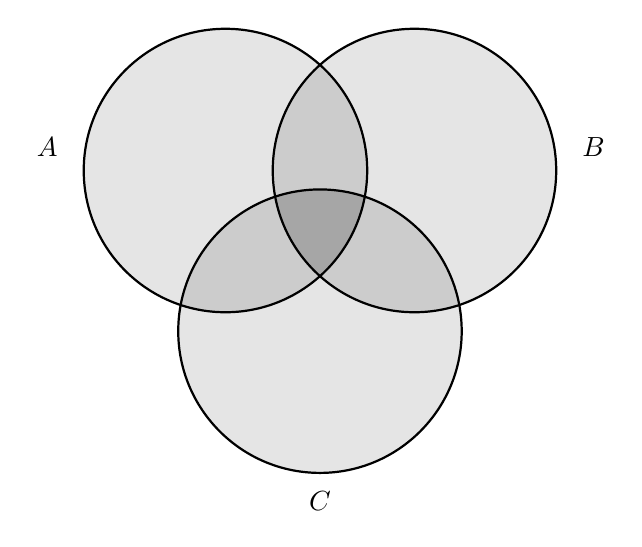
\begin{tikzpicture}[scale=1.2, thick]
\coordinate (A) at (0,0.7);
\coordinate (B) at (2,0.7);
\coordinate (C) at (1,-1);

\fill[gray!20] (A) circle (1.5);
\fill[gray!20] (B) circle (1.5);
\fill[gray!20] (C) circle (1.5);

\begin{scope}
  \clip (A) circle (1.5);
  \fill[gray!40] (B) circle (1.5);
\end{scope}

\begin{scope}
  \clip (A) circle (1.5);
  \fill[gray!40] (C) circle (1.5);
\end{scope}

\begin{scope}
  \clip (B) circle (1.5);
  \fill[gray!40] (C) circle (1.5);
\end{scope}

\begin{scope}
  \clip (A) circle (1.5);
  \clip (B) circle (1.5);
  \fill[gray!70] (C) circle (1.5);
\end{scope}

\draw[black] (A) circle (1.5) node[left=2cm, yshift=0.3cm] {$A$};
\draw[black] (B) circle (1.5) node[right=2cm, yshift=0.3cm] {$B$};
\draw[black] (C) circle (1.5) node[below=2cm, yshift=0.1cm] {$C$};
\end{tikzpicture}
\end{center}
\[
  |A \cup B \cup C| = |A| + |B| + |B| - |A \cap B| - |A \cap C| - |B \cap C| + |A \cap B \cap C|
\]
\begin{theorem}[Inclusion-exclusion Principle]
   Let $S_1, S_2, \ldots, S_n$ be finite sets. Then:
   \begin{align*}
     |S_1 \cup S_2 \cup \cdots \cup S_n| &= \sum_{|A| = 1} |S_A| - \sum_{|A| = 2} |S_A| + \sum_{|A| =  3} |S_A| - \cdots + (-1)^{n + 1} \sum_{|A| = n} |S_A| \\
                                         &= \sum_{r = 1}^{n} (-1)^{r + 1} \sum_{|A| = r} |S_A|
   \end{align*}
   Where $S_A = \bigcap_{i \in A} S_i$ and $\sum_{|A| = k}$ is taken over all $A \subseteq \{1, 2, \ldots, n\}$ of size k.
\end{theorem}
\begin{proof}
  Let $x \in S_1 \cup S_2 \cup \cdots \cup S_n$, say $x \in S_i$ for $k$ of the $S_i$ with $0 \leq k \leq n$.
  We want $x$ to be counted exactly once in the right hand side.

  The number of multi-indices with dimension 1 where $x \in S_A$ is just $k$ as $x$ was in $k$ of the sets.
  \[
    |\{A: |A| = 1 \text{ with } x \in S_A\}| = k
  \]
  The number of multi-indices with dimension 2 where $x \in S_A$ is $\binom{k}{2}$ as in this case $S_A$ is the intersection of two sets and there are $k$ choose $2$ ways of choosing two sets whose intersection will also contain $k$.
  \[
    |\{A: |A| = 2 \text{ with } x \in S_A\}| = \binom{k}{2}
  \]
  In general:
  \[
    |\{A: |A| = r \text{ with } x \in S_A\}| =
    \begin{cases}
    \binom{k}{r} & \text{ if } r\leq k \\
    0 & \text{ if } r > k
    \end{cases}
  \]
  Note that if $r > k$ then there are no such multi-indices as this would require $x$ to be in more that $k$ sets if it is to be in their intersection.

  As all terms with $r > k$ on the right hand side will be 0, the number of times $x$ is counted on the right hand side is then:
  \begin{align*}
    \sum_{r=1}^{k} (-1)^{r + 1} \binom{k}{r} &= k - \binom{k}{2} + \binom{k}{3} - \cdots + (-1)^{k + 1} \binom{k}{k} \\
    &= 1 - \left(1 - k + \binom{k}{2} - \binom{k}{3} + \cdots + (-1)^{k}\binom{k}{k}\right) \\
    &= 1 - (1 + (-1))^{k} \text{ (by Binomial Theorem)}\\
    &= 1
  \end{align*}
  So any $x \in S_1 \cup S_2 \cup \cdots \cup S_n$ is counted exactly once.
\end{proof}
\begin{remark}[Multi-Indicies]
  A multi-index can be thought of as an $n$-dimensional tuple of indices.
  That is $A = (\alpha_1, \alpha_2, \ldots, \alpha_n)$ where $\alpha_i$ are indices.
\end{remark}
\begin{example}
  With $|A| = 2$, $A$ is a subset of size two of $\{1, 2, \ldots, n\}$. So
  \[
    \sum_{|A| = 2} |S_A| = \sum_{|A| = 2} \abs{\bigcap_{i \in A} S_i }
  \]
  is the sum of all the sizes of all the different unions of two sets.
\end{example}
An equivalent formulation of the inclusion-exclusion principle is:
\[
  \abs{\bigcup_{i=1}^{n} S_i} = \sum_{r=1}^{n} (-1)^{r+1} \sum_{\substack{A \subseteq \{1, 2, \ldots, n\}\\ |A| = r}} \abs{\bigcap_{i \in A}^{} S_i}
\]
\begin{remark}
  We can also prove the inclusion-exclusion principle with indicator functions using the fact that if $A \subseteq X$ then:
  \[
    |A| = \sum_{x \in X} i_A(x)
  \]
\end{remark}
\end{document}
